\documentclass[conference]{IEEEtran}
\IEEEoverridecommandlockouts
% The preceding line is only needed to identify funding in the first footnote. If that is unneeded, please comment it out.
\usepackage{cite}
\usepackage{amsmath,amssymb,amsfonts}
\usepackage{algorithmic}
\usepackage{graphicx}
\usepackage{textcomp}
\usepackage{xcolor}
\def\BibTeX{{\rm B\kern-.05em{\sc i\kern-.025em b}\kern-.08em
    T\kern-.1667em\lower.7ex\hbox{E}\kern-.125emX}}
\begin{document}

\title{Title}

\author{\IEEEauthorblockN{Boris Stampf}
\IEEEauthorblockA{\textit{IT Security} \\
\textit{FH Technikum Wien}\\
Vienna, Austria\\
cs19m006@technikum-wien.at}
\and
\IEEEauthorblockN{Maximilian Wech}
\IEEEauthorblockA{\textit{IT Security} \\
\textit{FH Technikum Wien}\\
Vienna, Austria \\
cs19m020@technikum-wien.at}
}

\maketitle

\begin{abstract}
@TBA
\end{abstract}

\begin{IEEEkeywords}
artificial intelligence, neural networks, computer networks, network security
\end{IEEEkeywords}

\section{Introduction}
@Boris

\section{Feature Extraction}
@Boris

\section{Neural Network}
The created dataset will be used in the further course of this paper to build a neural network. With this it should be possible to detect anomalies in network traffic (e. g. DoS attacks) but also harmless data packets. This is a continuation of  \cite{max1}, in which an attempt was made to create a neural network for intrusion detection on the basis of the publicly available CSE-CIC-IDS2018 dataset  \cite{max2}. The knowledge gained at that time is used, the source codes are reused accordingly and slightly adapted to the new dataset. In principle, the performance of neural networks over different datasets is to be checked. The following scenarios will be considered:
\smallskip

Scenario 1) What performance can be achieved with a neural network when it is trained and tested with the dataset created in this work? 
\smallskip

Scenario 2) How well does the neural network created in Scenario 1 work when tested with the CSE-CIC-IDS2018 dataset  \cite{max2}? 
\smallskip

Scenario 3) How well does the neural network trained in \cite{max1} work when tested with the dataset created in this work?
\smallskip

It is suspected that there are differences in the intrusion detection datasets because, for example, cyber attacks are not always executed or recorded in the same way or the network infrastructure is structured differently. The aim is to determine how sensitive neural networks react to this and are thus dependent on the data with which they have been trained. This chapter is designed in such a way that the various steps for building up the neural network are first described and then the results obtained are examined in detail.

\subsection{Setup}
For the practical implementation, a notebook with 16GB RAM and a 2.7 GHz dual-core processor was used. This hardware was sufficient for the fulfillment of the task. The training of the neural network took about 4 hours. PyCharm Community Edition 2020.1 was used as a Python development environment on Windows 10. Packages were basically the same as in \cite{max1}. The Seaborn package 0.10.1 was also used to create heatmaps.

\subsection{Preprocessing}
This process is based on the one from\cite{max1}. This involves preparing the created dataset for training the neural network accordingly. A difference compared to \cite{max1} is that this time no headers were in the middle of the created CSV file. For this reason, the "skip\_rows" parameter did not have to be used in the "read\_csv" pandas function. In addition, identical entries in the dataset (duplicates) are also removed and a corresponding data type is specified for each feature. The conversion of the labels into a numeric format also takes place. At this point it should be noted that due to time constraints, not all types of attack from \cite{max2} could be reproduced in this work. This can be seen from the fact that some (numerical) labels are not represented in the created dataset. In the context of future work, the missing types of attack can be added. It is important that the labels in the created dataset must have the exact same numerical representation as in \cite{max1}. This means, for example, that benign network traffic must be labeled with "0" again. Furthermore, no types of attack were implemented in the context of this work that are not available in the CSE-CIC-IDS2018 dataset \cite{max2}. This is because the neural network from \cite{max1} could not recognize them and thus no performance comparison would be possible. For this reason, attacks from the CSE-CIC-IDS2018 dataset \cite{max2} were selectively reproduced. It should also be noted that in \cite{max1} some attacks of the publicly available dataset were not included.

\smallskip
The following Table \ref{table:overviewdatasets} provides an overview of both datasets:
\begin{table}[htbp]
\caption{Overview of the two datasets } 
\centering
\begin{tabular}{ | c | c | c | }
\hline
Label & \multicolumn{1}{|p{2cm}|}{\centering Number of data \\ points in the dataset  \\ created in this work}  & \multicolumn{1}{|p{2cm}|}{\centering Number of data \\ points in the \\  CSE-CIC-IDS2018 dataset \cite{max2}}\\
\hline
benign (0) & 63.264 & 10.180.908 \\
\hline
ddos attacks-loic-http (1) & Not available & 575.364 \\
\hline
ddos attack-hoic (2) & 193.729	& 198.861 \\
\hline
dos attacks-hulk (3) & Not available & 145.199 \\
\hline
bot (4) & Not available & 144.535 \\
\hline
ssh-bruteforce (5) & 29.182 & 94.048 \\
\hline
dos-goldeneye (6) & 7.368.370	 & 41.406 \\
\hline
dos attacks-slowloris (7) & Not available & 9.908 \\
\hline
ddos attack-loic-udp (8) & Not available & 1.730 \\
\hline
\end{tabular}
\label{table:overviewdatasets}
\end{table}

\newpage

While the CSE-CIC-IDS2018 dataset \cite{max2} has a total of 10,182,638 data points (6.41GB distributed over multiple CSV files), the dataset created in this work consists of 7,654,545 data points (4.1GB, only one CSV file). When looking at Table 1, it is noticeable that both datasets are unbalanced and there is one label for which comparatively many data points exist (dataset created in this work: "dos-goldeneye", CSE-CIC-IDS2018 dataset: "benign").
The preprocessing process of the final dataset takes about 10 minutes. This is comparatively faster than in \cite{max1}, which could be due to the smaller file size and the fact that the current dataset consists of only one CSV file (there is no need to merge several files). Finally, the dataset was divided into a training and a test set at a ratio of 80:20. While the former is used to train the neural network, the latter is used to determine the performance of the neural network (with data not used for training).

\subsection{Training the neural network}
After the preprocessing of the data has been completed, the next task is to train and test the neural network. The architecture recommended in \cite{max1} (three hidden layers with 69 neurons each) and the hyperparameters (Learn rate: 0. 0001, Optimizer: adam, Weight initialization: normal, Activation function: relu, Number of neurons per layer: 69, Epochs: 850, Batch size: 256) are reused. In addition, "MinMaxScale" was used to normalize the data and a weight value of 500 was set for benign" traffic. At this point it is worth mentioning that attempts have been made to adjust individual parameters such as the learn rate or the weight value of benign traffic in order to achieve a better result. However, this has not had any positive effects. Future work could deal with this in more detail and try to find optimal hyperparameters by an extensive gridsearch. Of course, this would require appropriate hardware resources.

\smallskip
Training of the neural network with the training set took 4 hours and was stopped after 129 epochs. As in \cite{max1}, "EarlyStopping" with a value of 50 epochs was used. This means that after 50 epochs without improvement, the learning process is terminated to avoid overfitting.

\subsection{Results}
In the further course of this chapter, the aim is to present and evaluate the results achieved. To determine how good the classifications of machine learning algorithms are, an appropriate measure is required. The following metrics are relevant \cite{max3}:
\smallskip 

Accuracy: How likely is the model to make a correct prediction?
\smallskip

Precision for class A: How likely is the classification to be correct if the model predicts class A?
\smallskip

Recall for class A: How much data of a class A can the model correctly predict?
\smallskip

Both the dataset created in this work and the CSE-CIC-IDS2018 dataset \cite{max2} are unbalanced (different amounts of data per class). For this reason, the use of Accuracy does not seem to be appropriate. If a very large amount of data were available for a class A and not for classes B and C, then the accuracy would be very dependent on class A. Instead, it is advisable to graphically display the classification results of the neural network in a confusion matrix and to calculate precision and recall respectively. The following text analyses the results of the three scenarios in the introduction:
Figure  \ref{fig:cm1} shows the result of the first scenario in which a neural network was trained and tested with the dataset created in this work. The classification results are largely good. However, it is noticeable, that only 62.5\% of all data of the "ssh-bruteforce" attack type can be correctly classified (comparatively low recall). The precision value for "benign" traffic is also comparatively lower, which means that it is only 86\% correct if the neural network predicts this class. All other precision and recall values are well over 95\%.

\begin{figure}[htbp]  
\centerline{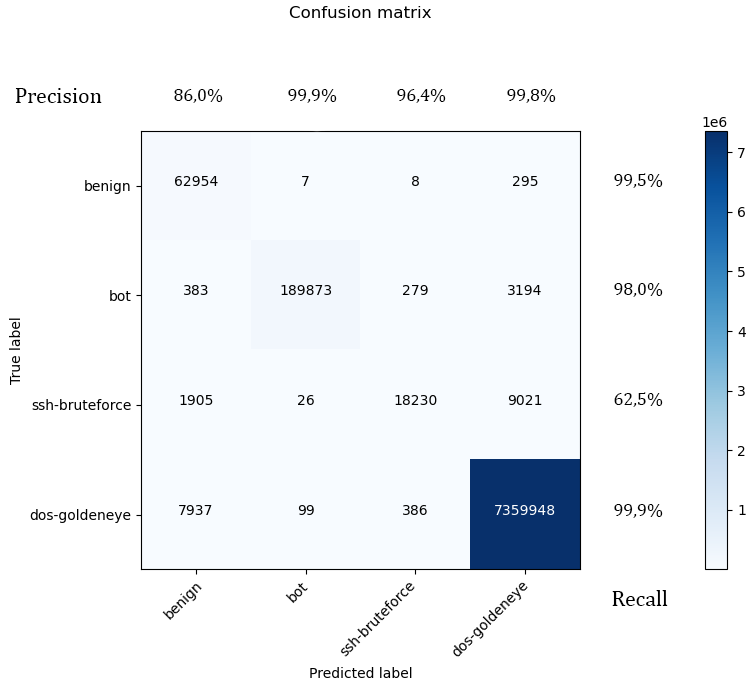
\includegraphics[scale=0.65]{NeuesModellNeueDaten.png}}
\caption{Confusion Matrix for Szenario 1}
\label{fig:cm1}
\end{figure}

Next, the neural network trained in Scenario 1 was reused and tested with the CSE-CIC-IDS2018 dataset \cite{max2}. There are many more classes (attack types) in this dataset than in the one used to train the neural network. Thus, the model would not be able to recognize these classes. For this reason, it is necessary to reduce the CSE-CIC-IDS2018 dataset \cite{max2} to the known four classes ("benign", "bot", "ssh-bruteforce" and "dos-goldeneye"). The reduced dataset is then used to test the neural network. The Confusion Matrix in Figure  \ref{fig:cm2} shows that the classification result is anything but good. On the positive side, the precision for benign traffic is very high, so if the model predicts this class, the prediction is 99.4\% correct. However, only 24.2\% of all data in this class can be correctly predicted. All other precision and recall values are or move around 0\%. It is worth mentioning that the "ssh-bruteforce" attack cannot be recognized correctly once. Scenario 1 already indicated a worse classification result for this class. Both "bot"- and "dos-goldeneye" attacks could be detected at least a few times, but to a very small extent. Overall, this suggests that there may be differences in the two datasets that significantly affect the classification outcome of the neural network. Thus, there is a suspicion that the machine learning model is overfitting.

\begin{figure}[htbp]  
\centerline{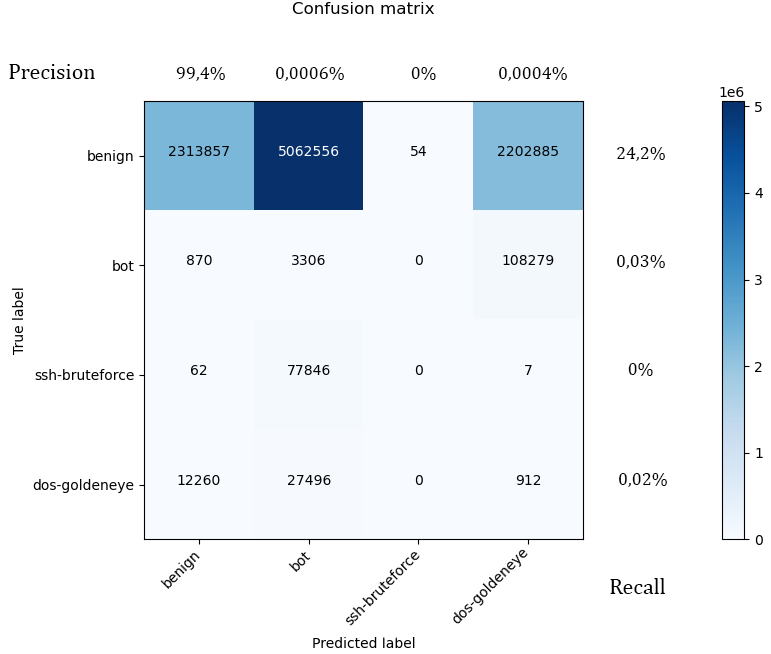
\includegraphics[scale=0.65]{NeuesModellAlteDaten.png}}
\caption{Confusion Matrix for Szenario 2}
\label{fig:cm2}
\end{figure}

In the third scenario, the neural network from \cite{max1}, which was trained with CSE-CIC-IDS2018 Dataset \cite{max2}, is now tested with the dataset of this work. This continues the low classification success (see Figure \ref{fig:cm3}). In the class "benign", 99.8\% of all data are correctly predicted (recall), but the precision is noticeable low (0. 008\%). This means that the neural network recognizes many data points as "benign", but these are mostly other classes. Conversely, this is the case with "bot", where only few data of this class are correctly recognized, but whenever the neural network recognizes this class, it is a correct prediction. All other precision and recall values are or move around 0\%. It is particularly noticeable that "bot"-, "ssh-bruteforce"- and "dos-goldeneye" attacks are mostly classified as benign traffic. Furthermore, it can be seen that "ssh-bruteforce"- and "dos-goldeneye" attacks cannot be correctly detected once; bot attacks can be correctly predicted nine times in total. This makes it clear how weak the classifications of the neural network trained in \cite{max1} are with the dataset created in this work. Also worth mentioning is that for some data points the classes "ddos attacks-loic-http", "dos attacks-hulk" and "dos attacks-slowloris" are predicted. These are not available in the dataset created in this work, but in the CSE-CIC-IDS2018 dataset \cite{max2}, with which the neural network was trained. For this reason, this is not surprising.

\begin{figure}[htbp]  
\centerline{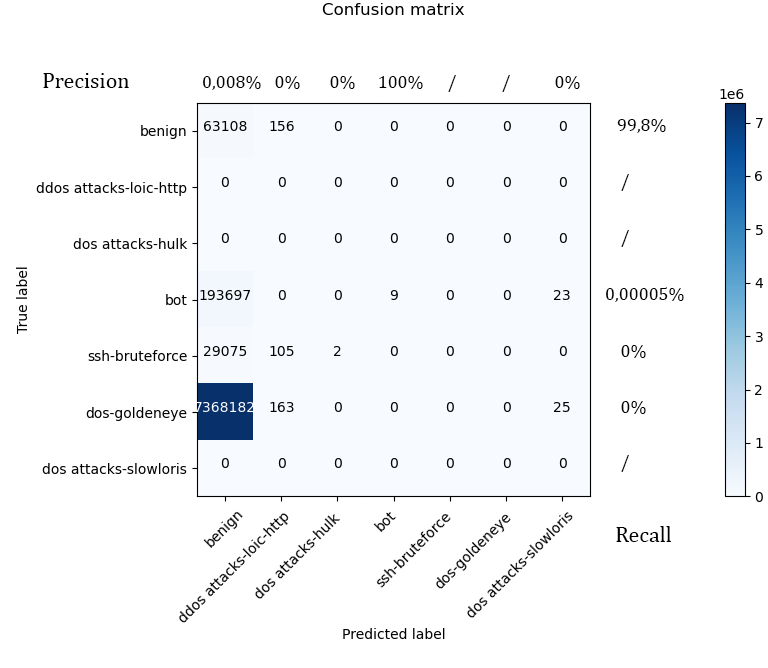
\includegraphics[scale=0.65]{AltesModellNeueDaten.png}}
\caption{Confusion Matrix for Szenario 3}
\label{fig:cm3}
\end{figure}

Scenarios 2 and 3 show that if in this context a neural network is tested with a different dataset than the one it was trained with, then the classification performance is poor. There can be many reasons for this. The suspicion, however, is that there are differences in the datasets and that this affects the predictions of the neural networks. One approach is to perform a correlation analysis. This makes it possible to determine the statistical relationship between two features (variables) of a dataset. The correlation coefficient is to be calculated, which indicates the strength of the correlation in the interval [-1.1]. A positive correlation means the larger the variable A, the larger the variable B. The opposite is the negative correlation, in which the larger the variable A is, the smaller the variable B. If the correlation coefficient is 0, this is called a neutral correlation and there is no relationship between the variables \cite{max4}. The idea is to determine the correlation between the features (variables) for each dataset individually. From this, graphical representations (heatmaps \cite{max5}) can be created in order to be able to compare whether correlation differences can be detected in the datasets. Since the number of features is high in both datasets, it makes sense to use only a subset of the features for the analysis. Thus, the correlation between the first 36 features is determined for both datasets. Figure \ref{fig:hm1} and Figure \ref{fig:hm2} each show the results for the two datasets. Clear differences are recognizable. It is worth mentioning that Figure \ref{fig:hm1} shows numerous negative correlations, which are not at all or hardly recognizable in Figure \ref{fig:hm2}. It is also noticeable that in Figure \ref{fig:hm2}, white lines occur, meaning that a feature in the dataset created in this work always has a value of zero. This shows that there are differences in the datasets. 

\begin{figure}[htbp]  
\centerline{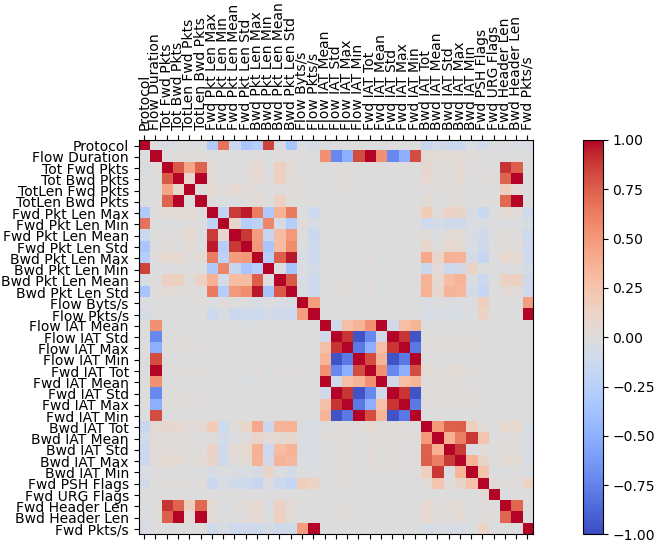
\includegraphics[scale=0.8]{Heatmap-AlteDaten-Filtered-0-35.png}}
\caption{Heatmap of the first 36 features of the CSE-CIC-IDS2018 Dataset}
\label{fig:hm1}
\end{figure}

\begin{figure}[htbp]  
\centerline{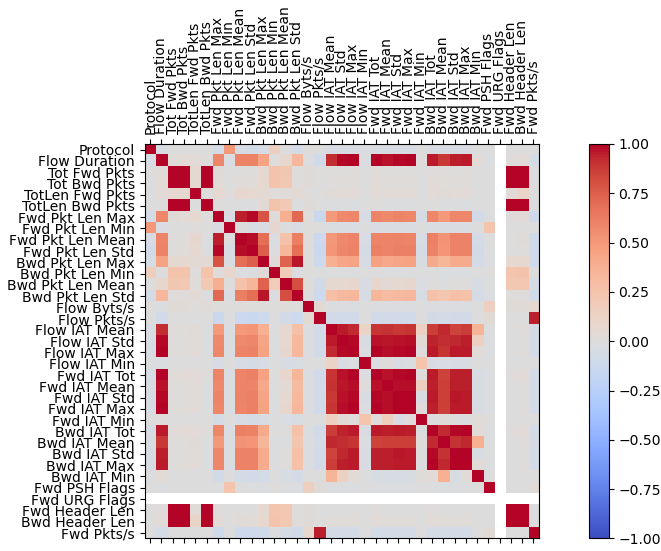
\includegraphics[scale=0.8]{Heatmap-NeueDaten-0-35.png}}
\caption{Heatmap of the first 36 features of the dataset created in this work}
\label{fig:hm2}
\end{figure}

\section{Conclusion}
In summary, the performance of neural networks in terms of intrusion detection over different datasets is rather mixed. If these machine learning algorithms are tested with the same dataset with which they were trained, the result is promising. Using another dataset for testing results in a poor classification performance. However, there is lots of potential for future research with neuronal networks in terms of intrusion detection. It seems useful to analyse in detail why the mentioned difficulties occur in the classification and which factors are relevant for the neural network. An intensive examination of the finding of optimal hyperparameters would also be desirable in the course of future work. Furthermore, it would also make sense to simplify the way classification is done. Instead, a simple classification like network traffic is “benign” or “not benign” would be conceivable. Moreover, it should be checked whether a better performance can be achieved with other machine learning algorithms.

\begin{thebibliography}{00}
\bibitem{max1} F. Ahrens, C. Cat and R. Freingruber, "A Neural-Network Approach for an Intrusion Detection System", FH Technikum, Vienna, 2019.
\bibitem{max2} I. Sharafaldin, A. H. Lashkari and A. A. Ghorbani, "Toward Generating a New Intrusion Detection Dataset and Intrusion Traffic Characterization", in 4th International Conference on Information Systems Security and Privacy (ICISSP), Portugal, 2018.
\bibitem{max3} D. Meyer, "Performance Assessment \& Tuning - Presentation slides", FH Technikum, Vienna, 2018.
\bibitem{max4} J. Brownlee, "How to Calculate Correlation Between Variables in Python", 3 June 2020. [Online]. Available: https://machinelearningmastery.com/how-to-use-correlation-to-understand-the-relationship-between-variables/. [Accessed 27 June 2020].
\bibitem{max5} S. Norena, "Finding Correlation Between Many Variables (Multidimensional Dataset) with Python", 26 April 2018. [Online]. Available: https://medium.com/@sebastiannorena/finding-correlation-between-many-variables-multidimensional-dataset-with-python-5deb3f39ffb3. [Accessed 27 June 2020].
\end{thebibliography}

\end{document}